\documentclass{article}

\usepackage[ngerman]{babel} % Deutsche Texte (Inhaltsverzeichnis)
\usepackage[utf8]{inputenc} % UTF8 für ÜÄÖ
\usepackage{hyperref} % Für Links
\usepackage{graphicx} % Für Bilder
\usepackage{amsmath} % mathe symbole
\usepackage{amssymb} % erweiterte math symbole
\usepackage{listings} % für Code
\usepackage{xcolor} % Für Code
\usepackage{tabularx} % für tabellen

\lstset{ %
language = C++,
 backgroundcolor=\color{black!5}, % set backgroundcolor
    basicstyle=\footnotesize,% basic font setting
}




%Deckblatt

\title{Sortieralgorithmen}
\author{Tobias Schneider, Fatih Kahraman}
\date{\today}



\pagenumbering{roman}
\begin{document}

% HDA FBI Logo
\begin{figure}

\includegraphics[scale = 1.5]{fbi_bild.png}
\end{figure}

\maketitle % setzt title author und date
\thispagestyle{empty} % Diese Seite ohne Seitenzahl
\newpage{}

\tableofcontents{}% 2 mal ausführen für richtige darstellung des Inhaltsverzeichnis!!!!!!!!!!!!!!!!!!!!!!
\setcounter{page}{1} % Seitenzahlzähler zurück auf 1 setzen
\newpage{}
\pagenumbering{arabic}


\section{Einleitung}
\subsection{Abstract}
\textbf{Sortieralgorithmen sind heutzutage nicht mehr wegzudenken. Ihre Benutzung ist essentiell für die Verwaltung von vielen Dateien. Sichtbar für den Benutzer wird es z.B. auf Shopping Webseiten, auf welchem man gewisse Artikel nach Wunsch anordnen kann. Wie und welches Sortieralgorithmus hier verwendet wurde, bleibt dem Kunden unbewusst. Interessant für den Entwickler ist die Stabilität und die Schnelligkeit des Sortieralgorithmusses. 
In dieser Seminararbeit werden wir uns auf ein Verfahren konzentrieren, mit dem die Laufzeit berechnet werden kann. Ebenso werden wir verschiedene Experimente durchführen, in dem wir unterschiedliche Testumgebungen(IDE) benutzen.
Um einen Überblick zu erschaffen, müssen wir uns mit den zahlreichen Eigenschaften eines Sortieralgorithmusses bekanntlich machen. Im Quelltext wird nachgeforscht, ob zusätzlicher Speicher benötigt wird und ob dies die Performance beeinträchtigt.
Die umfangreichen Versuche zeigen darauf, dass es keinen perfekten Sortieralgorithmus existiert. Wir veranschaulichen die Stärken und Schwächen der genannten Verfahren in unterschiedlichen Umgebungen.}
\subsection{Leser Fangen}
\subsection{Problem und Relevanz}

%\section{Hauptteil}
\section{Grundlagen}
\subsection{O-Notation}
Mithilfe der O-Notation, auch Landau-Notation gennant, wird eine Laufzeitberechnung anhand der gegebenen Eingabelänge n bestimmt. Dabei wird ein ungefähres Wachstumsverhalten des Algorithmus als mathematische Funktion definiert. Dies geschieht durch Analyse des Quellcodes und wird üblicherweise für drei Fälle durchgeführt: \cite{ONotation}\\ \\
\textbf {Worst-Case:} Es wird nach der maximalen Laufzeit des Algorithmus gesucht. Dies geschieht indem eine obere Schranke aufgestellt wird, über die die Laufzeit nicht steigt. Dieser Fall ist Sortieralgorithmus abhängig und kann nicht immer eine in umgekehrter Reihenfolge sortierte Liste sein.   \\
\textbf {Best-Case:} Stellt die minimale Laufzeit da und wird durch eine untere Schranke realisiert. Auch hier fällt die Laufzeit nicht unter die Schranke. Der Best-Case ist nicht immer eine bereits aufsteigend sortierte Liste sein.\\
\textbf {Average-Case:} Es wird eine durchschnittliche Laufzeit aufgestellt. \\ \\
\textbf{Vorteil der Landau-Notation} ist, dass sie komplett unabhängig von Hardware und Betriebssystem ist. Mit ihr kann man die Laufzeiten von Algorithmen miteinander vergleichen.\\
\textbf{Ein großer Nachteil} ist das die Funktionen nur angenähert sind und so nur eine grobe Einschätzung liefern.% Weiterhin existiert keine Berücksichtigung auf Speicher Allokationen oder Zeitdauer von  rekursive aufrufe.

\subsection{In-Place}
Diese Eigenschaft beschreibt ob der Algorithmus neben der zu sortierenden Liste noch weiteren Speicherplatz benötigt oder nicht. Eine Ausnahme ist der zwischenspeicher der beim tausch zweier Werte benötigt wird. Wenn der Algorithmus nur das Array und diesen zwischenspeicher verwendet wird er als In-Place bezeichnet. \cite{in-place}
\subsection{Stabilität}
Ein stabiler Algorithmus behält die Reihenfolge von äquivalenten Werten bei. Diese Eigenschaft ist bei Sortierung von Zahlen nicht relevant, aber sobald mehr Dateien damit zusammenhängen gewinnt diese Eigenschaft an relevanz. \cite{stability}
%\subsection{Heap/Stack Größe}
\subsection{Testumgebung}
Die Tests wurden auf einem Intel I5 Prozessor mit einer Taktfrequenz von 2,5 GHz ausgeführt. Zur Implementierung der Sortieralgorithmen wurde die Sprache C++, mithilfe der Entwicklungsumgebung Netbeans 8.2 mit dem GCC Compiler 4.9.3, benutzt.

\section{Sortieralgorithmen}
Sortierverfahren werden benutzt, um große Datensammlungen in einer bevorzugten Reihenfolge an zu ordnen. Heutzutage herrschen inzwischen eine Menge von Sortieralgorithmen, die ihre Vorteile in verschiedenen Gebieten der IT bekanntlich machen. Welches Verfahren wo benutzt werden soll, hängt von einer gewissen Anzahl von Kriterien ab.
Im Folgenden werden sechs populäre Sortieralgorithmen vorgestellt, wie sie Schritt für Schritt im Programm vorangehen.

\subsection{BubbleSort}
\subsubsection{Geschichte}
%\subsubsection{Pseudo-Code}
%void bubbleSort(T liste[], int anzahl) {
    %boolean swapped;
    %for (int i = 1; i < anzahl; i++) {
       % bool swap = false;
        %for (int j = 0; j < anzahl - i; j++) { 
           % if (liste[j] > liste[j + 1]) {
               % 	swap(j, j+1);
                	%swapped = true;}
        %}
        %if (!swapped) {
           % return;}
%}}
%\begin{lstlisting}

%func bubblesort( var a as array )
   % for i from 1 to N
       % for j from 0 to N - 1
      %     if a[j] > a[j + 1]
   %           swap( a[j], a[j + 1] )
%end func
%http://www.algorithmist.com/index.php/Bubble_sort
%\end{lstlisting} 
%Code von \cite{bubbleSortCode}.
\subsubsection{Vorgehensweise}
Idee: Größere Elemente steigen im Array nach rechts auf.\\ \\
Der BubbleSort ist ein Algorithmus der mit zwei ineinander verschachtelten Schleifen arbeitet. Die äußere Schleife definiert bis zu welchem Punkt die innere Schleife läuft. Die innere Schleife vergleicht das aktuelle Element mit dem darauf folgenden, und falls das aktuelle größer ist, werden diese beiden Elemente vertauscht.\\
Wenn die innere Schleife einen Durchlauf abgeschlossen hat, steht das größte Element am Ende und wird danach nicht mehr berücksichtigt. \\
Eine Besonderheit wurde noch hinzugefügt, es wird in einem Schleifendurchlauf mittels „swapped“ kontrolliert ob getauscht wurde. Falls nicht getauscht wurde, ist die Liste schon fertig sortiert und der BubbleSort wird abgebrochen. Mit diesem Trick ist der Best-Case O(n) möglich. 


\subsubsection{Eigenschaften}
\textbf{O-Notation:} Da bei einer bereits sortierten Liste keine vertauschungungen erfolgen , ist der BubbleSort nach einem Schleifendurchlauf fertig und beendet sich mit dem break. Beim Worst-Case werden beide Schleifen komplett durchlaufen was zu einer O-Notation von $n^{2}$ führt.
\begin{table}[h]
\centering
\begin{tabular}{lll}
	\hline
	\textbf{Best Case} & \textbf{Average Case} & \textbf{Worst Case} \\
	\hline
	O(n) & O($n^{2}$) & O($n^{2}$) \\
	\hline
\end{tabular}
\caption{O(Notation) des BubbleSorts \cite{ONotationen}}
\label{tab:bubbleSort}
\end{table}
\\\textbf{Best-Case} Der Best-Case des BubbleSorts ist eine bereits sortierte Liste. Der Algorithmus geht die Liste einmal durch und merkt es wurde nicht getauscht. Es erfolgt ein \"break\". Die O-Notation ist deshalb O(n).\\
\textbf{Worst-Case} Eine in falscher Reihenfolge sortierte Liste ist der Worst-Case des BubbleSorts. Da dadurch beide Schleifen komplett durchlaufen werden ist die O-Notation O($n^{2}$). \\ \\
\textbf{Stabilität} Da nur jeweils benachbarte Elemente mittels echt größer als verglichen und vertauscht werden, ist der BubbleSort ein stabiler Algorithmus \\ \\
\textbf{In-Place} Da der Algorithmus keine rekursiven aufrufe durchführt und lediglich zum vertauschen einen temporären Speicherplatz benötigt, arbeitet der Algorithmus mit O(1). \\




%\subsubsection{Testfälle}
%kommen bald!
%SOON TM

\subsection{InsertionSort}
\subsubsection{Geschichte}
%\subsubsection{Pseudo-Code}
%\begin{lstlisting}
%for i from 1 to N
 %  key = a[i]
   %j = i - 1
  % while j >= 0 and a[j] > key
     % a[j+1] = a[j]
     % j = j - 1
   %a[j+1] = key
%http://www.algorithmist.com/index.php/Insertion_sort
%\end{lstlisting}
%Code von \cite{InsertionSortCode}

\subsubsection{Vorgehensweise}
Idee: Einsortieren von Elementen in eine bereits sortierte Liste. \\ \\
Der InsertionSort arbeitet wie der BubbleSort mit zwei ineinander verschachtelten Schleifen.Die Anzahl der Elemente ist am anfang auf 2 Elemente festgelegt. Bei jedem äußeren Durchlauf wird die größe des Arrays um eins erhöht, bis zu seiner maximal größe. Dadurch wird immer ein Element zur bereits sortierten Liste hinzugefügt und an die richtige stelle einsortiert. Die bereits sortierten Elemente werde falls nötig nach hinten verschoben.

\subsubsection{Eigenschaften}
\textbf{O-Notation:}
\begin{table}[h]
\centering
\begin{tabular}{lll}
	\hline
	\textbf{Best Case} & \textbf{Average Case} & \textbf{Worst Case} \\
	\hline
	O(n) & O($n^{2}$) & O($n^{2}$) \\
	\hline
\end{tabular}
\caption{O(Notation) des InsertionSorts \cite{ONotationen}}
\label{tab:InsertionSort}
\end{table}
\\
\textbf{Best-Case} Der Best-Case des InsertionSorts ist eine bereits sortierte Liste. Da dann die Anzahl der verschiebungen null ist. Da die Äußere Schleife aber n mal aufgerufen wird und die innere auch ist hier die O-Notation O($n^{2}$). \\
\textbf{Worst-Case} Eine falsch herum sortierte Liste ist der Worst-Case. Ähnlich wie beim Best-Case werden die Schleifen durchlaufen. Es wird aber bei jedem durchgang maximal verschoben. Auch hier ist die O-Notation O($n^{2}$).\\ \\
\textbf{Stabilität:}  Es werden nur benachbarte Elemente miteinander verschoben falls ein Element echt größer ist. Es werden außerdem nur Elemente von links in das Array eingefügt. Dadurch ist die Stabilität gegeben.\\ \\
\textbf{In-Place:}  Der Algorithmus arbeitet nur auf der übergebenden Liste. Es wird nur ein zusätzlicher Speicher für das Vertauschen benötigt deshalb ist der InsertionSort O(1).\\


%\subsubsection{Testfälle}
%blargh
%SOON TM
\subsection{SelectionSort}
\subsubsection{Geschichte}
%\subsubsection{Pseudo-Code}
%\begin{lstlisting}
%void selectionSort(T liste[], int anzahl) {
 %   int k;
   % T temp;
    %for (int i = 0; i < anzahl; i++) {
       % k = i;
       % for (int j = i + 1; j < anzahl; j++) {
          %  if (liste[j] < liste[k]) {
             %   k = j;
            %}  }
       % swap(i,k)
          %  }}
%\end{lstlisting}
\subsubsection{Vorgehensweise}
Idee: Suche das kleinste Element und stelle es nach vorne. \\ \\
Mithilfe von zwei ineinander veschachtelter Schleifen wird der SelectionSort implementiert. Dabei wird das Array komplett durchlaufen um das kleinste Element darin zu finden. Danach wird das kleinste Element mit dem Element an der ersten Stelle vertauscht und der Startwert um 1 erhöht. Dies geschieht solange bis das Array schlussendlich sortiert wurde.
\subsubsection{Eigenschaften}
\textbf{O-Notation:}
\begin{table}[h]
\centering
\begin{tabular}{lll}
	\hline
	\textbf{Best Case} & \textbf{Average Case} & \textbf{Worst Case} \\
	\hline
	O($n^{2}$) & O($n^{2}$) & O($n^{2}$) \\
	\hline
\end{tabular}
\caption{O(Notation) des SelectionSorts \cite{ONotationen}}
\label{tab:SelectionSort}
\end{table}
\\
\textbf{Best-Case} Der Best-Case ist eine bereits sortierte Liste, da in diesem fall nicht getauscht werden muss. Es wird aber bei jedem einzelnen Durchgang das Array komplett durchlaufen. \\
\textbf{Worst-Case} Ähnlich wie beim Best-Case werden die Arrays jedesmal Durchlaufen. Es muss aber bei jedem Durchgang getauscht werden.\\ \\
\textbf{Stabilität:} Der SelectionSort ist kein Stabiler Algorithmus. Bei der Wahl des kleinsten Elements wird zwar die Stabilität gewährleistet, aber beim vertauschen wird das vorderste Element mit dem kleinsten vertauscht. Hier kann das vorderste hinter ein Element gebracht werden, was die gleiche größe besitzt.   \\
\\
\textbf{In-Place:}  Der SelectionSort arbeitet auf dem Array und benötigt zusätzlich nur einen Tauschspeicher. Er hat deshalb einen Wert von O(1). \\
%\subsubsection{Testfälle}
%soon
%SOON TM

\subsection{MergeSort}
\subsubsection{Geschichte}
%\subsubsection{Pseudo-Code}
%Sehr Groß
\subsubsection{Vorgehensweise}
Idee: Teile das Array in der mitte in zwei hälften bis das Array nur noch ein Element behält. Füge danach die teile wieder sortiert zusammen. \\
\\
Der MergeSort baut auf dem Teile und Hersche Prinzip auf. Er besteht aus zwei teilen:
\\ \\
\textbf{MergeSort:} Das Array wird in der Mitte geteilt und danach wird der MergeSort Rekursiv für diese Teilmengen aufgerufen. Dies geschieht solange bis das übergebene Array genau die größe 1 besitzt. Es ist zu beachten das hier auf dem Array gearbeitet wird. Es werden nur neue Start und Endpunkte des Arrays übergeben. \\
\textbf{Merge: } Sobald ein Teilbereich nicht mehr geteilt werden kann, werden diese Elemente wieder zusammengefügt. Dabei wird der Inhalt aus den beiden Teilarrays in temporäre Arrays gespeichert und dann der größe nach in das Ursprungsarray zurückgeschrieben. Die temporären Arrays werden danach wieder gelöscht. 


\subsubsection{Eigenschaften}
\textbf{O-Notation:}
\begin{table}[h]
\centering
\begin{tabular}{lll}
	\hline
	\textbf{Best Case} & \textbf{Average Case} & \textbf{Worst Case} \\
	\hline
	O(n log n) & O(n log n) & O(n log n) \\
	\hline
\end{tabular}
\caption{O(Notation) des MergeSorts \cite{ONotationen}}
\label{tab:MergeSort}
\end{table}
\\
\textbf{Best-Case:} Der Best-Case ist eine bereits sortierte Liste. Der entscheidende Faktor ist das zusammenfügen. Es wird erst die linke hälfte mit der rechten hälfte verglichen und jeweils nur die linke hälfte wird einsortiert. Da nun keine Elemente in der Linken hälfte sind, kann nun der Inhalt der rechten hälfte ohne vergleiche in das Array zurückgeschriebenen werden.\\
\textbf{Worst-Case:} Der Worst-Case ist eine Liste bei der immer abwechselnd ein Wert von der Linken hälfte und danach ein Wert von der Rechten hälfte einsortiert wird. Dadurch muss immer verglichen werden.\\ \\
\textbf{Stabilität:}  Der MergeSort ist ein Stabiler Sortieralgorithmus. Beim zusammenfügen wird das Linke Array mit kleiner gleich  mit dem Rechten Array verglichen. Dadurch werden die von der größe her gleichen Elemente im Linken Element bevorzugt. Es ist somit nicht möglich ein Element im linken zu überholen.\\
\\
\textbf{In-Place:} Der MergeSort arbeitet nicht In-Place, da der Tauschspeicher jeweils zweimal die hälfte der Teilmengen ist. Da der Algorithmus von Unten nach Oben neue Arrays erstellt ist der zusätzliche Speicherplatz O(n).   \\
%\subsubsection{Testfälle}
%soon
%SOON TM
\subsection{QuickSort}
\subsubsection*{Geschichte}
%\subsubsection*{Pseudo-Code}
\subsubsection*{Vorgehensweise}
Idee: Finde Stellvertreter Element. Setze links vom Element alles was kleiner ist. Setze rechts alles was größer ist. Führe dies Rekursiv für linke und rechte hälfte aus.\\
\\
Der QuickSort baut auf dem Prinzip von Teile und Hersche auf. Er besteht aus zwei teilen:\\ \\
\textbf{Partition:} Es wird ein Stellvertreter Element aus der Liste ausgewählt. Dies kann: das erste Element, das letzte Element, das Element in der mitte oder der Median aus erstes, mitte und letztes sein.\\ Danach werden die Elemente die kleiner sind links davon und Elemente die größer sind rechts davon positioniert.\\
\textbf{QuickSort:} Nun wird die linke und rechte hälfte rekursiv mit dem QuickSort wieder aufgerufen. %Das Pivot wird in der rechten hälfte hinzugefügt, da es sein kann, dass das Pivot nicht an der richtigen stelle steht.



\subsubsection*{Eigenschaften}
\textbf{O-Notation:}
\begin{table}[h]
\centering
\begin{tabular}{lll}
	\hline
	\textbf{Best Case} & \textbf{Average Case} & \textbf{Worst Case} \\
	\hline
	O(n log n) & O(n log n) & O($n^{2}$) \\
	\hline
\end{tabular}
\caption{O(Notation) des QuickSorts \cite{ONotationen}}
\label{tab:QuickSort}
\end{table}
\\
\textbf{Best-Case:} Der Best-Case des QuickSorts ist Pivot abhängig. Das Pivot Element ist der Punkt wo das Array aufgeteilt wird. Man möchte deshalb das das Pivot Element in der mitte ist um eine aufteilung in zwei möglichst gleichgroße hälften zugewährleisten. Zusätzlich werden keine vertauschungen durchgeführt. Dies entspricht bei Pivot Element Mitte einer sortierten Liste.\\
\textbf{Worst-Case:} Der Worst-Case ist  $n^{2}$. Er entsteht wenn das Pivot Element jeweils das Erste oder Letzte Element ist. Dadurch wird vom Array immer nur ein Element abgezogen, was im endeffekt einem Sortieralgorithmus mit zwei ineinander verschachtelter Schleifen gleicht.\\ \\
\textbf{Stabilität:} Der QuickSort ist kein stabiler Sortieralgorithmus. Beim Anwenden von Partition werden die Elemente vertauscht und es kann vorkommen das gleiche Elemente beim kopieren die reihenfolge vertauschen. \\
\\
\textbf{In-Place:} Es wird auf dem Array gearbeitet. Der Speicherverbrauch ist O(1), wegen dem Tauschspeicher.  \\
%\subsubsection*{Testfälle}
%SOON
%SOON TM
\subsection{HeapSort}
\subsubsection*{Geschichte}
%\subsubsection*{Pseudo-Code}
\subsubsection*{Vorgehensweise}
Idee: Erstellen eines Binärbaums. Größtes Element steht immer in der Wurzel. Stelle es an die letzte Stelle des Arrays und verringer die Arraygröße um eins. Führe dies rekursiv durch bis das Array sortiert ist.\\
\\
Der HeapSort besteht aus zwei Funktionen:\\\\
\textbf{Heapify:} Mithilfe der Heapify Funktion wird das Array von unten nach oben durchwandert. Dabei wird das größte Element aus Knoten und derren Linken und Rechten Kind im Knoten gespeichert. \\
\textbf{HeapSort:} Wenn Heapify abgeschlossen ist, steht das größte Element in der Wurzel. Nun wird dieses Element an die letzte stelle des Arrays kopiert und anschließend wird die größe des Arrays um eins verringert. Danach wird Heapify erneut aufgerufen.\\
\subsubsection*{Eigenschaften}
\textbf{O-Notation:}
\begin{table}[h]
\centering
\begin{tabular}{lll}
	\hline
	\textbf{Best Case} & \textbf{Average Case} & \textbf{Worst Case} \\
	\hline
	O(n log n) & O(n log n) & O(n log n) \\
	\hline
\end{tabular}
\caption{O(Notation) des HeapSorts \cite{ONotationen}}
\label{tab:HeapSort}
\end{table}
\\
\textbf{Best-Case:} Der Best-Case des HeapSort wird durch minimale vertauschungen beim ausführen von heapify erreicht. Dabei sollte so wenig wie möglich vertauscht werden. Dies ist durch eine Liste mit nur äquivalenten Werten der Fall, da in diesem Fall nicht vertauscht wird. \\
\textbf{Worst-Case:} Der Worst-Case wird durch maximale vertauschungen beim ausführen der Heapify Funktion. \\\\
\textbf{Stabilität:} Da Beim vertauschen das Element in der Wurzel mit dem letzten vertauscht wird, kann es dadurch zu instabilen vertauschungen kommen.  \\
\\
\textbf{In-Place:} Das Array wird intern zu einem Binärbaum auf dem dann sortiert wird. Diese Umformung wird nur mathematisch durchgeführt wodurch kein zusätzlicher Speicherplatz benötigt wird. Es wird zum vertauschen aber ein temporärer zwischenspeicher benötigt. \\
%\subsubsection*{Testfälle}

%\subsubsection{Vorstellung}
%Im folgenden Abschnitt werden wir uns hauptsächlich die Sortieralgorithmen im Detail anschauen. Für unsere Recherche haben wir uns auf drei grundlegende Verfahren eingeschränkt: Bubblesort, Quicksort und Mergesort. Der wohl am häufigsten verwendete Sortieralgorithmus ist der Quicksort. Seine Entstehung blickt weit zurück bis in die 60er Jahre und seither wird der Quicksort von vielen Forschern untersucht. Einer seiner haupt Eigenschaften ist es, dass er in-place abläuft, also keinen weiteren Speicher benötigt, um die Sortierung durchzuführen. Der Grunde, wieso Quicksort so schnell ist, ist, dass seine innere Schleife sehr kurz ist und somit einfach optimiert werden kann. Für die Sortierung von n Elementen wird im Durchschnitt n log (n) Operationen erfordet. Der Nachteil des Algorithmus ist, dass er rekursiv ist, also im worst-case braucht er $n^{2}$  Operationen. Ausgehend von diesen Behauptungen aus dem Netz, werden wir Tests durchführen, um zu schauen, in welchen Gebieten oder unter welchen Umständen diese genannten Aussagen gelten.


%\subsubsection{Pseudo Code}
%\subsubsection{Eigenschaften}
%Wie sind die O-Notation, In-Place, Stabilität zu diesem SA
%\subsubsection{Testfälle}
%Worst Case, Average Case, Best Case, nearly sorted, festplattenart, genug Speicher, zuwenig Speicher, unterschiedliche Datentypen - Integer versus Klassenobjekte

\newpage
\subsection{Evaluierung}
In den vorangegangenen Kapiteln wurden die Grundlagen gelegt. In dem nun folgenden Kapitel geht es um die empirische überprüfung der bereits vorgestellten Sortieralgorithmen.
Zum Einstieg in die Evaluation betrachten wir erst einmal die unterschiedlichen Funktionstypen und derren Wachstum.

\begin{figure} [h]
\centering
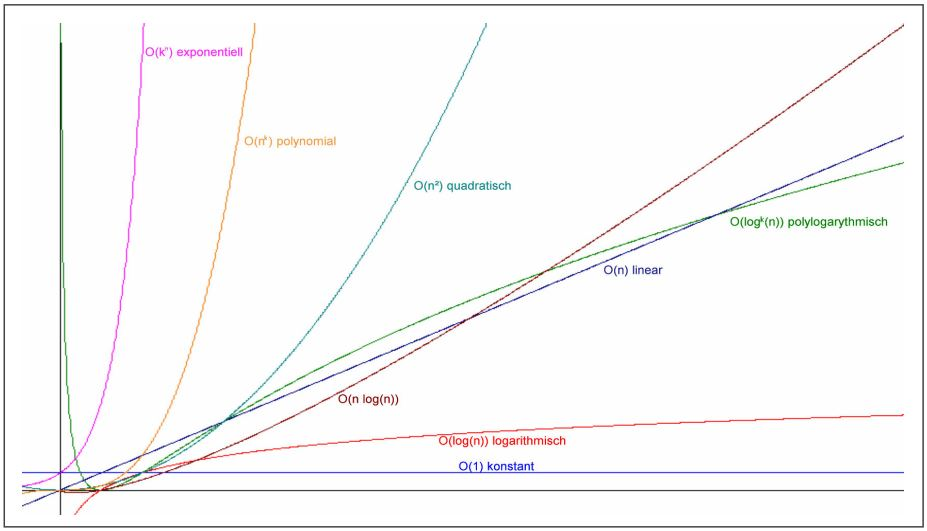
\includegraphics [width=\linewidth]{OWachstum.JPG} \label{fig:WachstumONotation}
\caption{Überblick der einzelnen Funktionen und derren Verlauf \cite{bild2006rehn}}
\end{figure}
Es wird sofort deutlich, dass die lineare und die n log n Funktionen ein deutlich niedrigeres Wachstum besitzen als die quadratische. 

\begin{table}[h]
\centering
\begin{tabular}{llll}
	\hline
	\textbf{Algorithmus} & \textbf{Best Case} & \textbf{Average Case} & \textbf{Worst Case} \\
	\hline
	BubbleSort & O(n) & O($n^{2}$) & O($n^{2}$) \\
InsertionSort & O(n) & O($n^{2}$) & O($n^{2}$) \\
SelectionSort & O($n^{2}$) & O($n^{2}$) & O($n^{2}$) \\
MergeSort & O(n log n) & O(n log n) & O(n log n) \\
QuickSort & O(n log n) & O(n log n) & O($n^{2}$) \\
HeapSort & O(n log n) & O(n log n) & O(n log n) \\
	\hline
\end{tabular}
\caption{O(Notation) der vorgestellten Algorithmen \cite{ONotationen}}
\label{tab:HeapSort}
\end{table}
Nun wäre es aber fahrlässig nur ahand der O-Notation einen Algorithmus auszuwählen. Denn wie im Kapitel zur O-Notation bereits erwähnt, werden konstanten entfernt.  

\subsubsection{Testfälle}
Um die Algorithmen untereinander zu vergleichen wurden einige Testfälle definiert.\\

\textbf{Zufalls-Werte:} Den einzelnen Algorithmen wurden die glechen Zufallszahlen übergeben und die Zeit gemessen bis diese die Liste sortiert haben.
\begin{table}[h]
\centering
\begin{tabular}{llllll}
\hline
\textbf{BubbleSort} & \textbf{SelectionSort} & \textbf{InsertionSort} & \textbf{QuickSort} & \textbf{MergeSort} & \textbf{HeapSort}  \\
\hline
34793,6 & 14644 & 12765,4 & 15,8 & 46,4 & 31,4 \\
\hline
\end{tabular}
\caption{Ergebnisse von Zufallswerten in Milisekunden(Durchschnittswerte)}
\label{tab:random}
\end{table}
\\An diesem Test erkennt man relativ schnell das die logarithmischen Algorithmen einen riesigen Vorteil gegenüber den quadratischen Algorithmen besitzen wenn es um zufällig sortierte Listen geht.\\


\textbf{Sortierte:} Es wird eine bereits sortierte Liste den einzelnen Sortieralgorithmen übergeben. Dies ist der Best-Case vom BubbleSort , InsertionSort, QuickSort(mit Pivot Element in der Mitte) und dem MergeSort.
\begin{table}[h]
\centering
\begin{tabular}{llllll}
\hline
\textbf{BubbleSort} & \textbf{SelectionSort} & \textbf{InsertionSort} & \textbf{QuickSort} & \textbf{MergeSort} & \textbf{HeapSort}  \\
\hline
$<1$ & 14640,6 & $<1$ & 6,4 & 31,2 & 34 \\
\hline
\end{tabular}
\caption{Ergebnisse von bereits Sortierter Liste in Milisekunden(Durchschnittswerte)}
\label{tab:sorted}
\end{table}
%
\\An diesem Beispiel erkennt man die stärke von O(n) im vergleich zu Logarithmischen Algorithmen. Der QuickSort muss keine vertauschungen durchführen weswegen er

\textbf{Absteigend Sortiert:} Den Algorithmen wird eine absteigend Sortierte Liste übergeben. Dies ist der Worst-Case des BubbleSorts, InsertionSort und SelectionSorts.
\begin{table}[h]
\centering
\begin{tabular}{llllll}
\hline
\textbf{BubbleSort} & \textbf{SelectionSort} & \textbf{InsertionSort} & \textbf{QuickSort} & \textbf{MergeSort} & \textbf{HeapSort}  \\
\hline
32427,8 & 15290,6 & 30072,2 & 9,2 & 31,2 & 40,8 \\
\hline
\end{tabular}
\caption{Ergebnisse von abgsteigend Sortierter Liste in Milisekunden(Durchschnittswerte)}
\label{tab:inverseSorted}
\end{table}
\\ %testfehlt



\subsubsection{Vergleich der Ergebnisse}
\subsubsection{Relevanz der O-Notation}
\subsubsection{Wie wichtig sind weitere Kriterien}
In-Place, Stabilität, Speicherplatz ...

\section{Schluss}
%\subsection{Fazit}
\subsection{Zusammenfassung und Ausblick}
\subsubsection{Fazit}
\subsubsection{Anwendungstipps}

\section{Literaturverzeichnis}

%\bibliography{mySA_Bib}
\bibliographystyle{ieeetr}
\bibliography{../BibTex/Sortieralgorithmen.bib}

%\section{Anhang} %Vllt später verwenden


\end{document}